\label{sec:kuramoto}

\subsection{Definition}
The problem of having a naive viewpoint on the subject of synchronization is that one may believe that every different coupling situation would require its own treatment. This may stem from the fact that one may be focusing too much on the differences rather then the similarities which are found in all synchronous systems.  In this project we want to use the model of oscilators that was first introduced by Kuramoto in ~\cite{book:kura}. The most common form is given by the following system of ODEs:
\[
\dot{\theta_i} = \omega_i + \sum_{j = 0}^{N - 1}{A_{i, j}\sin({\theta_j - \theta_i}}) + b_i \sin(\Omega(t) - \theta_i)
\]
In this equation
\begin{itemize}
	\item $\theta_i$ is the phase of the $i\textsuperscript{th}$ oscillator, 
	\item $N$ the number of oscilators, 
	\item $\omega_i$ is the natural frequency of the $i\textsuperscript{th}$ oscillator, 
	\item $A$ is the matrix of coupling coefficients of the system, 
	\item $\Omega(t)$ is the phase of an external driver to the system and
	\item $b$ is the vector of coupling coefficients to the external driver
\end{itemize}

In the Kuramoto oscilator model the main object of study is the phase of $N$ different so-called Kuramoto oscilators, $\theta_0$ to $\theta_{N - 1}$. It should be noted that one usually looks at this modulo $2 \pi$. Each oscilator oscilates at its own natural frequency $\omega_i$. However they are also influenced by the different other oscilators as well as by an external driver to the system. The observation of the other oscilations is represented by the periodic $\sin$ function. How strong each oscilator is influenced by the others and the external drivers is measured by the so-called coupling coefficients $A_{i, j}$ and $b_i$ respectively. 

\subsection{The Coupling matrix and associated network topology}

We can easily see from the notation above that we can consider the coupling coeffients $A_{i, j}$ as a square matrix $A$ of size $N$. Similarly we can consider the coupling to the external driver as a vector $b$ of length $n$. 

It turns out that if we take a symmetric matrix $A$ the system exhibits very interesting behaviour that can be related to another interpretation of $A$. A symmetric matrix containing only zeros and ones can naturally be seen as the adjacency matrix of an undirected, finite graph. In an adjacency matrix the elements indicate whether pairs of vertices are connected via an edge or not, i.e. if the value is $1$ there is an edge, otherwise there is not. This information can then be used to reconstruct the graph from the matrix. 

When solving the system this natural interpretation of $A$ is very useful to understand the dynamics. A typical plot generated when simulating the system can be found in Figure~\ref{fig:adjacencymatrix}. On the top is the graph that is created from an adjacency matrix $A$. Each vertex of the system represents a single oscilator. On the bottom is a plot of the phases of the oscilators of the system over time. 

\begin{figure}[h]
\centering
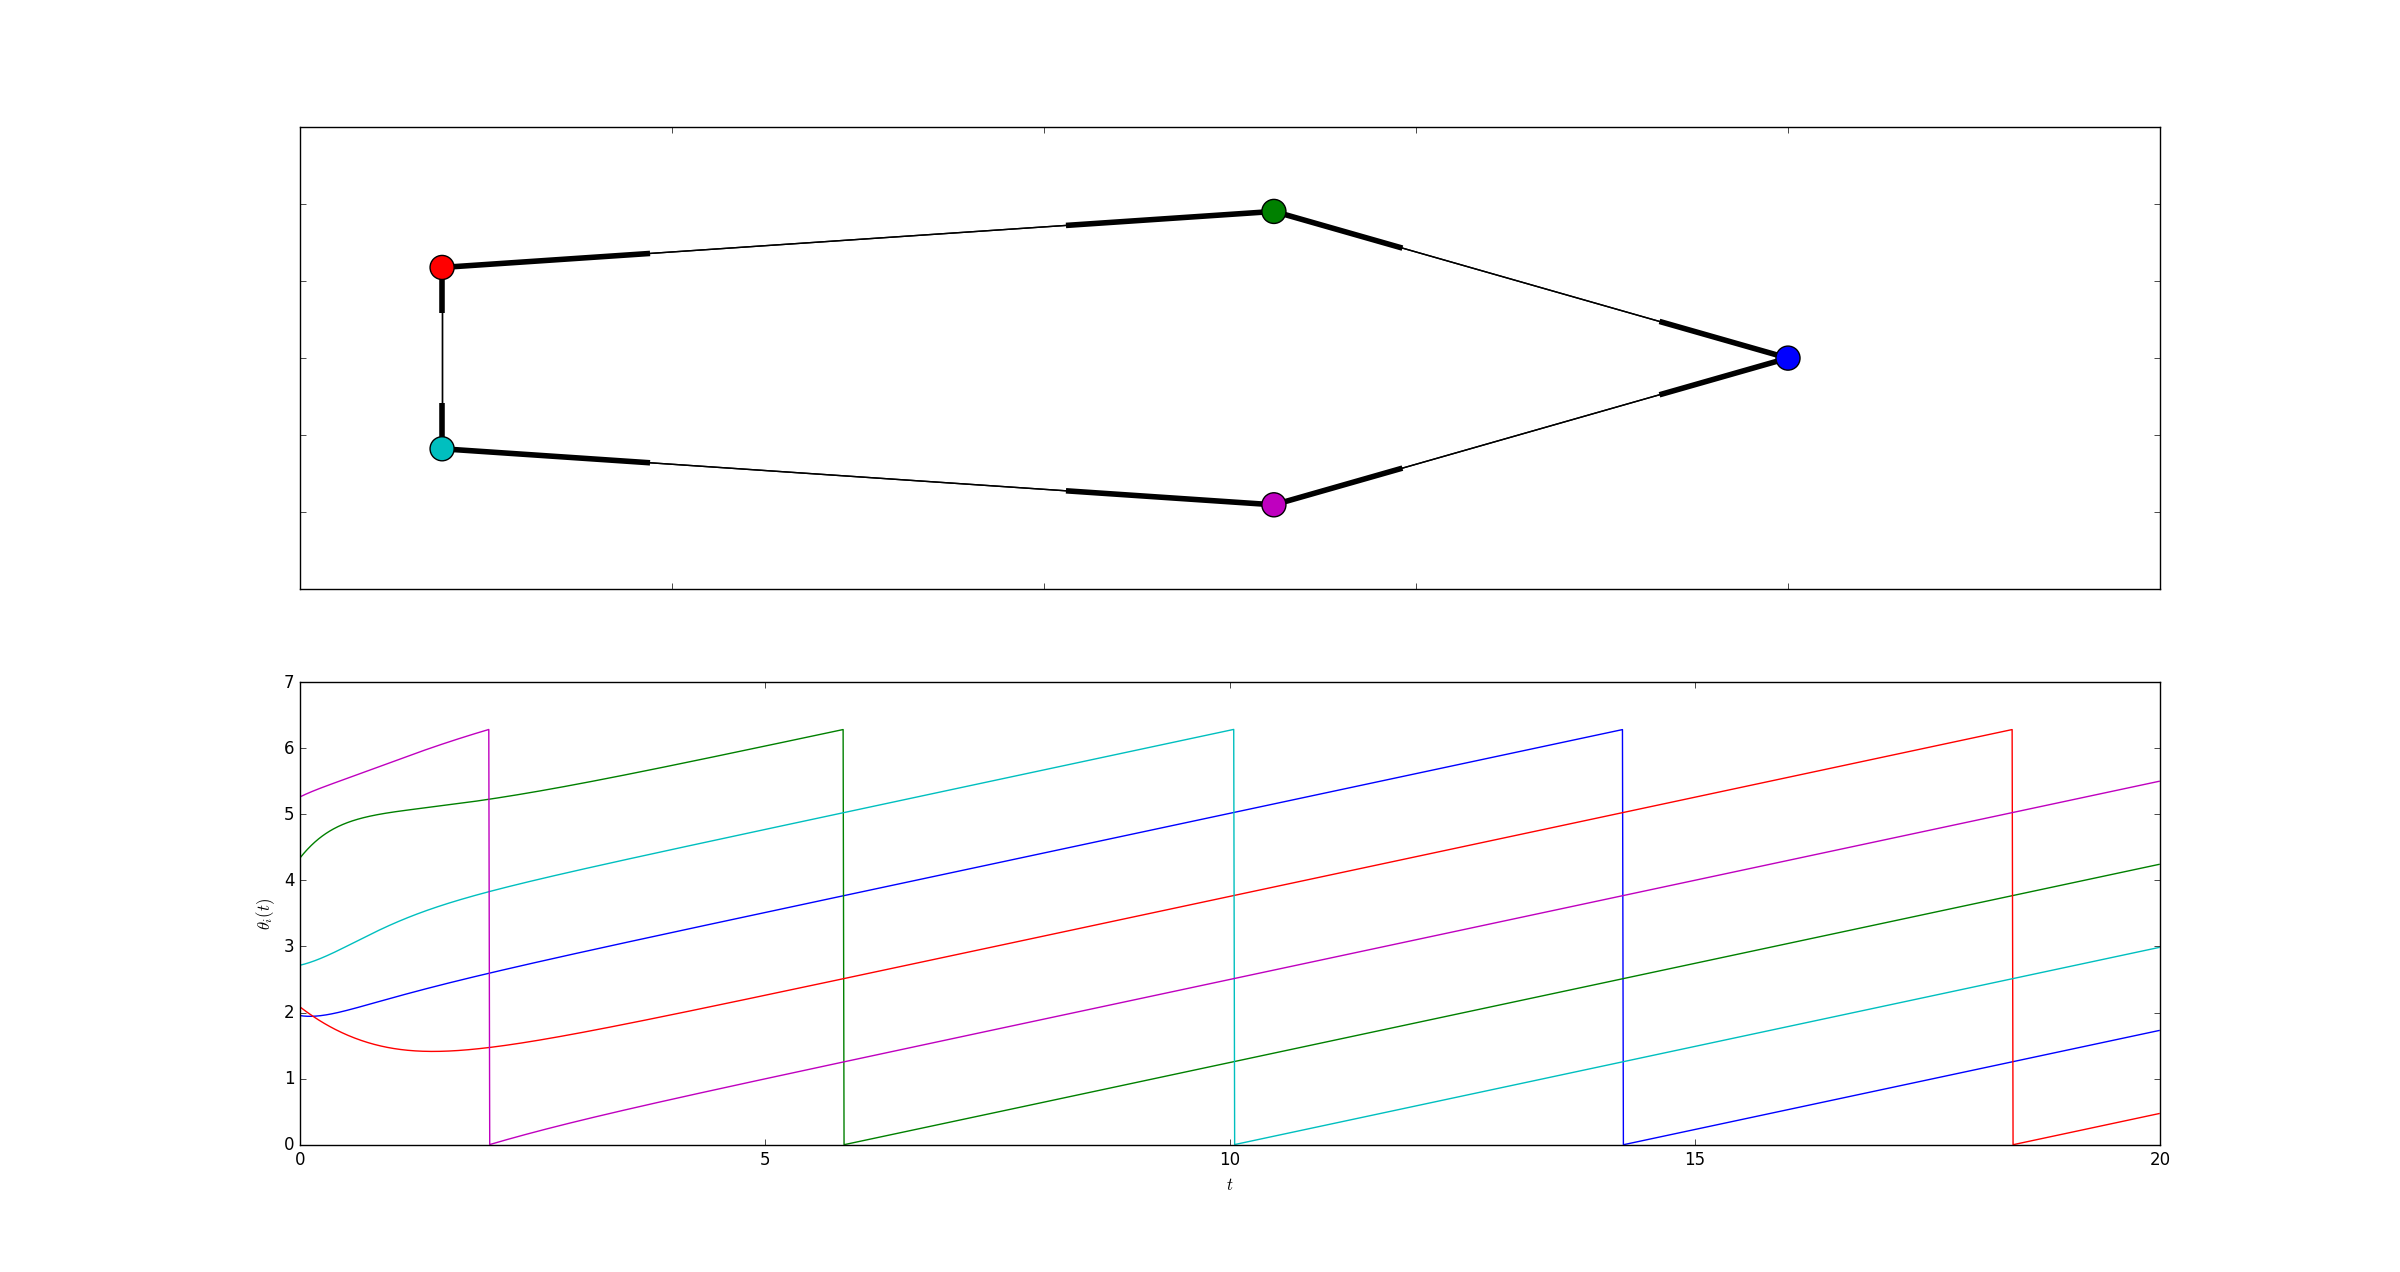
\includegraphics[width=\textwidth]{imgs/examplefigure}
\caption{A typical plot of a topology and output of the system}
\label{fig:adjacencymatrix}
\end{figure}

\subsection{Implementation of the system}
We have implemented a simulation of this system using Python3. Our implementation uses the python packages Numpy and Scipy and in particular leverages the standard ODE solver functionality provided. Our code is very modular and consists of four main parts: 

\begin{enumerate}
	\item A simulator of the system, found in ``oscilator.py''. This takes the parameters for the ODE and runs a simulation of the system given some initial values. 
	\item Some plotting code, found in ``plotter.py'', which takes the output of the system and makes plots like the ones that can be found in the various Figures in this report. 
	\item Some code that generates adjacency matrices for specific graphs, found in ``graph\_generators.py''. 
	\item the main code of the system (found in ``code.py'') which utilises the components above and runs the entire simulation. 
\end{enumerate}

The following code line illustrates the gist of how we used the NumPy package to compute the $\sin$ of the phase differences and the standard ode solver to numerically estimate the solution.
\begin{lstlisting}
if (self.A[i, j] != 0) and (i != j):
s.append('(%s)*np.sin(theta[%s] - theta[%s])' % (self.A[i, j], j, i))

if self.B[i] != 0:
s.append('(%s)*np.sin((%s)*t - theta[%s])' % (self.B[i], self.OMEGA, i))

sol = odeint(self.to_equation(), y0, t, *args, **kwargs)
\end{lstlisting}
Basically, we just append the calculated values into an array and later solve that using the ODE solver. 